\documentclass[11pt]{article}   	% use "amsart" instead of "article" for AMSLaTeX format
\usepackage{amsmath}
\usepackage{geometry}                		% See geometry.pdf to learn the layout options. There are lots.
\usepackage{tikz}
\usepackage{lipsum}
\usepackage{float}
\geometry{letterpaper}                   		% ... or a4paper or a5paper or ... 
\usepackage{setspace} % This package can be used to control the spacing
%\geometry{landscape}                		% Activate for rotated page geometry
%\usepackage[parfill]{parskip}    		% Activate to begin paragraphs with an empty line rather than an indent
\usepackage{graphicx}				% Use pdf, png, jpg, or eps§ with pdflatex; use eps in DVI mode
								% TeX will automatically convert eps --> pdf in pdflatex		
\usepackage{amssymb}
\usepackage{listings}
\usepackage{titlesec}
\let\oldsection\section
\renewcommand{\section}{\clearpage\oldsection}
\usepackage{xcolor}

\definecolor{codegreen}{rgb}{0,0.6,0}
\definecolor{codegray}{rgb}{0.5,0.5,0.5}
\definecolor{codepurple}{rgb}{0.58,0,0.82}
\definecolor{backcolor}{rgb}{0.95,0.95,0.92}

\definecolor{boxes}{rgb}{0.68, 0.85, 0.9} % define a light blue color

\setlength{\parskip}{1em} % add space between paragraphs

\lstdefinestyle{mystyle}{
    backgroundcolor=\color{backcolor},   
    commentstyle=\color{codegreen},
    keywordstyle=\color{magenta},
    numberstyle=\tiny\color{codegray},
    stringstyle=\color{codepurple},
    basicstyle=\ttfamily\footnotesize,
    breakatwhitespace=false,         
    breaklines=true,                 
    captionpos=b,                    
    keepspaces=true,                 
    numbers=left,                    
    numbersep=5pt,                  
    showspaces=false,                
    showstringspaces=false,
    showtabs=false,                  
    tabsize=2
}
\lstset{style=mystyle}

%\usepackage{blindtext}
%\usepackage{showframe}
%\renewcommand*\ShowFrameColor{\color{red}}
%\renewcommand{\arraystretch}{1.2}

%SetFonts

%SetFonts


\title{%
\ \\
\ \\
Xandeum: An L1 Smart Contract Platform with Scalable Blockchain-Based Storage \\
\ \\
\large INTERMEDIATE DRAFT v0.5}
\author{
{\rm Bernie Blume}\\
bernieb@xandeum.com
}

%\date{}							% Activate to display a given date or no date

\renewcommand*\contentsname{Summary}

\begin{document}
\maketitle
%\section{}
%\subsection{}

\maketitle

\ \\

\subsection*{Abstract}
This paper introduces Xandeum, a Layer-1 smart contract platform with an integrated, scalable, blockchain-based decentralized storage solution.

Today, the underperformance of storage solutions compared to conventional server-based applications presents a significant obstacle to the broader adoption of Web3. Xandeum's on chain storage solution will be the catalyst to realize the most consequential societal shifts of the 21st century, i.e., the empowerment of the user. Xandeum lays the foundation, facilitating the development and operation of storage-enabled decentralized apps (sedApps).

Xandeum blurs the line between applications designed for the blockchain (Web3) and those hosted on servers leveraging data center or cloud based storage solutions (Web2). Web2 applications have access to high-speed, high-capacity centralized storage solutions allowing for dynamice creation, reading, updating, and deletion (CRUD) of data. Xandeum is the Web3 CRUD solution adding censorship-resistance and tamper-proof (immutability) that is effecient, scalable, secure, and fully integrated into the smart contract platform. Xandeum is to storage what what other Layer-1 block chain solutions are to the CPU.

Borrowing from an industry leading Layer-1 smart contract solution, Xadeum inherits and extends its scalability even while adding its External Global Grouped Storage (EGGS) storage layer solution while avoiding economic scaling challenges. Xandeum is designed from the ground up to be economical even while scaling to from today's exabyte challenges to tomorrow's yottabyte. Xandeum achieves these milestones by adopting, adapting, and improving upon proven stratgies pioneered from other storage focused block chains, while smartly applying lessons learned to overcome security, scalability, and economic challenges each of them have failed to overcome in part or whole.

Xandeum's architecture facilitates seamless adoption, allowing developers to smoothly transition to Xandeum's storage solution. Xandeum has achieved this by embracing the Move programming language, allowing the same global storage operators to be used for both account and EGGS storage. Compatiblity sits at the heart of Xandeum's commitment to developers and individuals alike, minimizing friction in the transition from Web2 data center or cloud storage-based applications to Xandeum's Web3 decentralized storage solution.

\clearpage
\tableofcontents
\clearpage

\section{Design Goals}
\subsection{Boost Self-Determination of the Individual}
One of Xandeum's foremost design objectives is to boost the self-determination of the individual, a concept that sits at the core of decentralized technology. This aim transcends conventional use cases and focuses on a broader societal shift that lies at the heart of the blockchain revolution.

Self-determination, as opposed to determination by foreign forces, has been a common theme for humanity for ages, and can even be traced back to evolution in general. Foreign forces can be tribal leaders, modern governments, the need to spend the day hunting in order to survive tomorrow, and much more. The following figure illustrates the point, using $\mathcal{D}_{S}$ as the degree of collective self-determination in society, on a scale of 0 (totally controlled by external forces) to 1 (ideal self-determination and self-realization).

\ \\

\begin{figure}[H]
\noindent
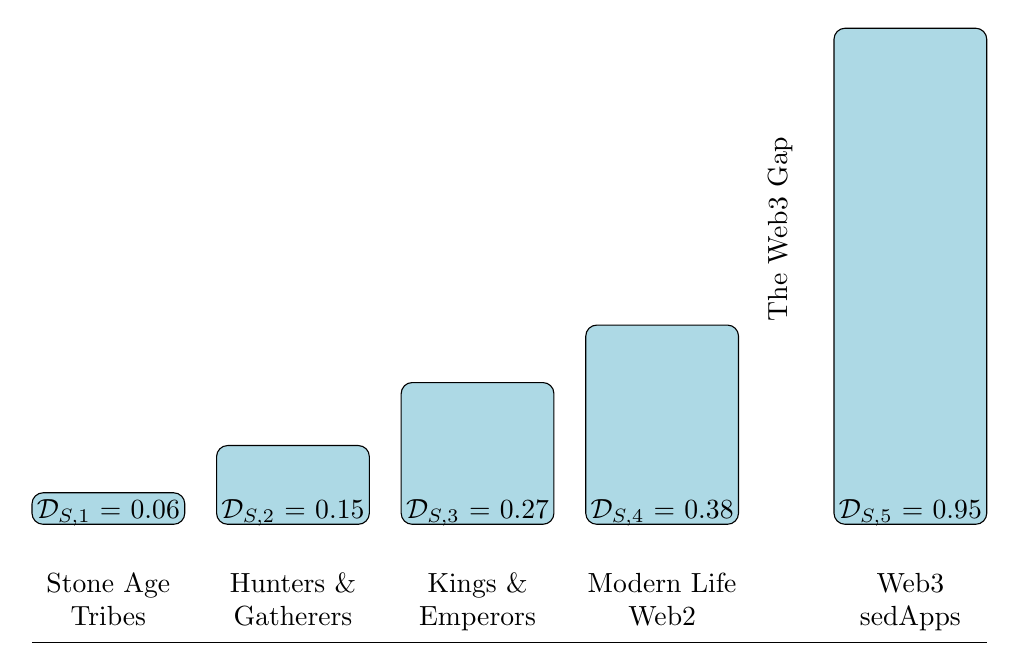
\begin{tikzpicture}
    \pgfmathsetmacro{\bigspacing}{0.1*\textwidth/1pt} % larger space, 10% of text width
    \pgfmathsetmacro{\spacing}{(0.2*\textwidth-\bigspacing)/3/1pt} % normal space, (20% of text width - larger space) divided by 3
    \pgfmathsetmacro{\rectanglewidth}{0.8*\textwidth/5/1pt} % rectangle width, 80% of text width divided by 5
    
    \draw[fill=boxes,draw=black,rounded corners] (0*\rectanglewidth+0*\spacing pt,0) rectangle ++(\rectanglewidth pt,0.4cm);
    \node[at={(0*\rectanglewidth+0*\spacing pt+0.5*\rectanglewidth pt, -0.15cm)}, anchor=south] {$\mathcal{D}_{S,1}$ = 0.06};
    \node[below=0.5cm,align=center] at (0*\rectanglewidth+0*\spacing pt+0.5*\rectanglewidth pt,0) {Stone Age \\ Tribes};

    \draw[fill=boxes,draw=black,rounded corners] (1*\rectanglewidth+1*\spacing pt,0) rectangle ++(\rectanglewidth pt,1cm);
    \node[at={(1*\rectanglewidth+1*\spacing pt+0.5*\rectanglewidth pt, -0.15cm)}, anchor=south] {$\mathcal{D}_{S,2}$ = 0.15};
    \node[below=0.5cm,align=center] at (1*\rectanglewidth+1*\spacing pt+0.5*\rectanglewidth pt,0) {Hunters \& \\ Gatherers};

    \draw[fill=boxes,draw=black,rounded corners] (2*\rectanglewidth+2*\spacing pt,0) rectangle ++(\rectanglewidth pt,1.8cm);
    \node[at={(2*\rectanglewidth+2*\spacing pt+0.5*\rectanglewidth pt, -0.15cm)}, anchor=south] {$\mathcal{D}_{S,3}$ = 0.27};
    \node[below=0.5cm,align=center] at (2*\rectanglewidth+2*\spacing pt+0.5*\rectanglewidth pt,0) {Kings \& \\ Emperors};

    \draw[fill=boxes,draw=black,rounded corners] (3*\rectanglewidth+3*\spacing pt,0) rectangle ++(\rectanglewidth pt,2.53cm);
    \node[at={(3*\rectanglewidth+3*\spacing pt+0.5*\rectanglewidth pt, -0.15cm)}, anchor=south] {$\mathcal{D}_{S,4}$ = 0.38};
    \node[below=0.5cm,align=center] at (3*\rectanglewidth+3*\spacing pt+0.5*\rectanglewidth pt,0) {Modern Life \\ Web2};
    
    % Add rotated text
    \node[rotate=90, above] at (4*\rectanglewidth+3.5*\spacing pt+0.5*\bigspacing pt, 3.75cm) {The Web3 Gap};

    \draw[fill=boxes,draw=black,rounded corners] (4*\rectanglewidth+3*\spacing+\bigspacing pt,0) rectangle ++(\rectanglewidth pt,6.3cm);
    \node[at={(4*\rectanglewidth+3*\spacing+\bigspacing pt+0.5*\rectanglewidth pt, -0.15cm)}, anchor=south] {$\mathcal{D}_{S,5}$ = 0.95};
    \node[below=0.5cm,align=center] at (4*\rectanglewidth+3*\spacing+\bigspacing pt+0.5*\rectanglewidth pt,0) {Web3 \\ sedApps};

    \draw (0, -1.5cm) -- (\textwidth, -1.5cm); % Draw a horizontal line at the bottom of the figure, 1.5cm below the bottom of the rectangles
\end{tikzpicture}
\caption{Collective Degree of Self-Determination $\mathcal{D}_{S,i}$ over time.}
\label{fig:my_label}
\end{figure}

We then define the collective degree of determination by foreign forces, $\mathcal{D}_{F}$, as
\begin{equation}
\mathcal{D}_{S} + \mathcal{D}_{F} = 1 
\end{equation}

The liberating power of evolutionary step $i$, $\mathcal{L}_{\mathit{i}}$, follows this equation:
\begin{equation}
\mathcal{D}_{F,i} = \mathcal{D}_{F,i-1} \cdot \frac{1}{\mathcal{L_{\mathit{i}}}}
\end{equation}

Our hypothesis is that all major evolutionary steps have increased collective self-determination, thus

\begin{equation}
\forall i = 1, 2, 3, \ldots, \infty, \quad \mathcal{L}_{\mathit{i}} > 1
\end{equation}

Xandeum's key design goal is to maximize $\mathcal{L}_{\mathit{i}}$, the liberating power of the next, blockchain-induced evolutionary step that humanity is taking. Of all possible Xandeum solutions $\mathcal{X}_{j}$, with $\mathcal{L(\mathcal{X}_{j})}$ representing the liberating power of solution $\mathcal{X}_{j}$ over the web2-based status quo, we pick solution $\mathcal{X}_{J}$, where

\begin{equation}
J = \arg \max_{j} \mathcal{L(\mathcal{X_j)}}
\end{equation}

Self-determination or the ability to control one's own destiny, as it is interpreted here, pertains to the power of individuals to own, control, and benefit from their data. This is a sharp departure from the prevailing Web2 paradigm, where data is predominantly controlled by centralized entities such as corporations or governments. The advancement of decentralized technologies and Web3 has brought us to the precipice of a paradigm shift, where individuals regain control and derive the full value from their data.

Xandeum furthers this vision by creating a Layer-1 platform that not only enables the development and operation of decentralized applications but also provides a robust, scalable, and efficient storage solution. In conventional server-based systems, programs have unrestricted access to vast and high-speed storage, allowing them to create, read, update, and delete data freely. This is not commonly the case with existing blockchain solutions.

By offering a blockchain-based storage layer that rivals the performance of traditional servers, Xandeum places power back in the hands of the individual. This blockchain-based storage layer is censorship-resistant and tamper-proof, giving individuals greater control over their data. In addition, the scalability and efficiency of Xandeum's storage solution make it an economically viable option for users.

Xandeum's design incorporates the proven reliability of blockchain technology, such as Solana's smart contract layer and the innovative EGGS (External Global Grouped Storage) system. This ensures that the platform can handle the vast volumes of data that individuals and decentralized applications generate.

The usage of the Move language by default reduces the barrier to entry for developers and promotes the further creation of applications that favor individual empowerment. The consistent use of Move's global storage operators for both the Accounts storage and the EGGS simplifies the development process, making the system more accessible to individual users and developers.

Xandeum's design embodies the idea of individual empowerment. It bridges the gap between the capabilities of conventional server-based systems and blockchain solutions, creating a platform where individuals have unprecedented control over their data. The advent of Xandeum is a significant stride toward a decentralized future where individuals are the true custodians of their data.

\subsection{Removing Web3 Roadblocks}
Presently, the broader transition towards a decentralized internet, or Web3, faces significant technological barriers that inhibit the development and implementation of storage-enabled decentralized apps (sedApps). These challenges present sizable roadblocks for startups aiming to bring Web3 analogs of popular Web2 applications like Airbnb and eBay to fruition.

The foremost challenge is the limited and expensive storage capabilities of existing blockchain solutions. Traditional blockchain systems lack the capacity for vast, efficient data storage, especially when compared with conventional server-based systems. This limitation restricts the extent to which applications can be decentralized, forcing reliance on off-chain storage solutions or centralized databases, which defeats the purpose of developing on a decentralized platform.

Another key hurdle is the challenge of scalability. As Web3 applications grow in usage and complexity, the demand for scalable storage solutions that can handle vast quantities of data becomes increasingly urgent. Unfortunately, contemporary blockchains struggle to scale economically, with costs often ballooning uncontrollably with increased data storage.

The technical proficiency required to develop on the blockchain is another considerable roadblock. The lack of a user-friendly interface or a universally accepted programming language makes it difficult for developers to transition to blockchain development, particularly for those who are new to the field.

Xandeum aims to dismantle these roadblocks through its innovative design. By introducing an efficient, scalable, blockchain-based storage layer, Xandeum delivers a solution that rivals the performance of conventional servers. The storage layer is integrated into a Layer-1 smart contract platform, enabling developers to build robust and fully decentralized applications.

Xandeum's scalable storage solution, powered by EGGS (External Global Grouped Storage) and a fork of Solana's smart contract layer, is engineered to handle large volumes of data economically, making it viable for projects developing ambitious Web3 applications. The storage solution is not only efficient and secure but is also resistant to censorship and tampering, underscoring the platform's commitment to a decentralized Web3 ecosystem.

Moreover, Xandeum mitigates the entry barrier for developers by adopting the Move language as its default programming language. Move's global storage operators are used consistently across Xandeum's platform for both Accounts storage and the EGGS, simplifying the development process and making the transition to blockchain development less daunting for developers.

Xandeum is designed to eliminate the roadblocks hampering the growth of Web3, providing developers with the tools necessary to bring their visions of decentralized applications to life. This approach clears the path for the creation of Web3 counterparts of popular Web2 applications, marking a critical step towards a fully decentralized internet.

\subsection{Frictionless Adoption}
Ensuring frictionless adoption of new technologies is a vital aspect of promoting their use and facilitating a successful transition. Xandeum acknowledges this necessity and, as a core design principle, has embedded mechanisms to foster easy and seamless integration into its platform.

Adoption is made effortless through Xandeum's use of the Move language as its default programming language. Move offers an approachable and powerful language for developers, providing consistency and stability for both the Accounts layer, which is based on Solana's accounts, and the EGGS layer (External Global Grouped Storage). The use of the same global storage operators across these layers simplifies the development process, significantly reducing the complexity and learning curve for developers transitioning to the decentralized storage solution. This is a remarkable departure from the intricate, often confusing patterns that prevail in other blockchain environments.

Moreover, Xandeum eliminates the necessity of negotiating individual storage deals—a cumbersome process that is common in other decentralized storage solutions like Sia and Filecoin. Instead, Xandeum's blockchain-based storage solution is straightforward, with storage provision and management integrated into the Layer-1 platform, thereby reducing transactional friction and enhancing the user experience.

The exceptional speed and performance of Xandeum's platform also contributes to frictionless adoption. By leveraging a modified version of Solana and an efficient, purpose-built EGGS layer, Xandeum delivers a scalable and high-performing solution that can comfortably handle the demands of storage-enabled decentralized apps (sedApps), no matter the scale of their operations.

Scalability is central to the design of Xandeum, engineered to ensure the platform can accommodate the vast quantities of data generated by decentralized applications and individual users alike. This scalability doesn't compromise the platform's economic viability; rather, it enhances it. As the system scales, it remains efficient and affordable, which is crucial for startups and individual developers sensitive to operational costs.

The issue of cost-effectiveness is further addressed through Xandeum's dynamic fee structure for both smart contract transactions and storage provisions. By adjusting fees based on market conditions, Xandeum offers a responsive and fair cost model, alleviating the financial burdens typically associated with blockchain storage and transactions.

Xandeum's design principles encompass and address the essential components for frictionless adoption: ease of use, seamless integration, speed, scalability, and affordability. By committing to these principles, Xandeum ensures that the transition to decentralized storage and the development of sedApps on its platform is as smooth as possible, reducing the barriers to entry for a new generation of Web3 applications.

\section{Smart Contracts Layer}
\subsection{Permissioned Fork of Solana}
Xandeum's smart contract layer is built upon a permissioned fork of Solana, a design decision underpinned by our unique funding model and commitment to community engagement. Unlike many blockchain startups, Xandeum chose not to pursue traditional venture capital in its early phases. Instead, it introduced a novel Solana-based crowdfunding platform known as "NodeStore" to sell licenses for its validator software to its community. This innovative funding model not only fosters a vibrant and invested community but also has proven very successful in supporting Xandeum's growth.

The permissioned nature of Xandeum's Solana fork is integral to this funding model. By incorporating a closed-source permission layer, Xandeum can ensure that only licensed software operators can validate transactions. Despite this permissioned feature, Xandeum harnesses the full power and scalability of the Solana blockchain for its smart contract layer, contributing to a highly efficient, performant, and secure platform. Any modifications to the Solana codebase that do not implicate the permission layer are made open source, reflecting Xandeum's commitment to transparency and community involvement.

The choice to base the smart contract layer on Solana stems from a careful comparison of smart contract chains and their alignment with Xandeum's design goals. Among the competing platforms, Solana was identified as the most promising due to its superior scalability, performance, and architectural robustness. Moreover, our team's experience operating the Bitoku Validator—a high-performance Solana validator—for about a year provided invaluable insights into Solana's capabilities and potential enhancements, further confirming Solana as the ideal choice.

The permissioned fork of Solana serves as the foundation of Xandeum's smart contract layer. It combines the best of Solana's attributes with Xandeum's unique permission layer, creating an efficient, scalable, and secure platform that is funded and maintained by an engaged community of license-holders. This design decision not only supports our commitment to individual empowerment and frictionless adoption but also illustrates the innovative approaches Xandeum is taking to achieve its ambitious goals.

\subsection{Use of the Move Language}
A critical component supporting our design goals is the adoption of the Move language, an innovative programming language for the implementation of smart contracts. With its robust safety features and approachability, Move contributes significantly to the overall efficiency and security of the Xandeum platform.

The representation of global storage according to the Move Book_{cite}, in pseudocode, is as follows:

\ \\
\begin{lstlisting}[caption=Global Storage in Move]
struct GlobalStorage {
    resources: Map<(address, ResourceType), ResourceValue>
    modules: Map<(address, ModuleName), ModuleBytecode>
}
\end{lstlisting}
\ \\

This represents the global storage structure as a forest composed of trees rooted at an account address. Each address serves as a storage space for both resource data values and module code values. As shown in the pseudocode, each address can contain at most one resource value of a given type and one module with a specified name.

\ \\
\phantom{~}
\begin{table}[!h]
\begin{center}
\begin{tabular}{p{0.4\textwidth}p{0.2\textwidth}p{0.2\textwidth}}
\hline
\textbf{Operation} & \textbf{Description} & \textbf{Aborts?} \\ \hline
move\_to$<$T$>$(\&signer,T) & Publish T under signer.address & If signer.address already holds a T \\ \hline
move\_from$<$T$>$(address): T & Remove T from address and return it & If address does not hold a T \\ \hline
borrow\_global\_mut$<$T$>$(address): \&mut T & Return a mutable reference to the T stored under address & If address does not hold a T \\ \hline
borrow\_global$<$T$>$(address): \&T & Return an immutable reference to the T stored under address & If address does not hold a T \\ \hline
exists$<$T$>$(address): bool & Return true if a T is stored under address & Never \\ \hline
\end{tabular}
\caption{\label{movesto}Move's Global Storage Operators.}
\end{center}
\end{table}
\ \\
Move programs can create, delete, and update resources in the global storage using Move's five global storage operators.

Xandeum offers the developer two of these structures, one for the Solana accounts storage, and one for the EGGS layer. Through this approach, incorporating EGGS into the code to develop real, storage-enabled web3 dApps is finally a seamless developer experience.

The above instructions offer Move a powerful capability to manage global storage, contributing significantly to the flexibility and functionality of smart contracts written in this language. With its careful design and well-defined operations, Move allows for a more efficient and safer manipulation of resources, aligning perfectly with the design goals of Xandeum.

\subsection{Storage Follows Control}
An important principle guiding the design and architecture of Xandeum is "Storage Follows Control". This principle encapsulates our strategic approach to developing a blockchain that facilitates the development of storage-enabled web3 dApps, known as sedApps.

Many existing storage chains are primarily designed for standalone storage. They are exceptional at storing and retrieving data in a decentralized manner, but they often lack the native features and compatibility necessary to facilitate the seamless development of sedApps. This is where Xandeum differentiates itself. It is not just a storage chain, but rather an integrated solution designed specifically for the creation of web3 applications.

The primary goal of Xandeum is to accelerate the adoption of web3 technology. To achieve this, we have focused on making the development process as familiar and intuitive as possible for dApp developers. Developers are already familiar with writing smart contracts, which form the basic building blocks of dApps. As such, Xandeum's architecture is designed to naturally extend this process by easily incorporating the External Global Grouped Storage (EGGS) layer into the development of these smart contracts.

In the world of web2, developers would simply open a file, write to it, and their application would have access to storage. Xandeum seeks to replicate this ease of access in the web3 space. Through the EGGS layer, smart contracts written on Xandeum can interact with storage as simply as web2 developers interact with files.

In effect, the principle of "Storage Follows Control" ensures that the control logic contained within smart contracts has a seamless and integrated method of accessing and managing storage, mirroring the ease and simplicity of web2 development. By simplifying the process of developing sedApps and bringing web3 development closer to established web2 practices, Xandeum aims to usher in the next wave of decentralized application development.

\section{Storage Layer}
\subsection{External Global Grouped Storage (EGGS) Overview}
At the heart of the Xandeum blockchain lies the External Global Grouped Storage (EGGS) layer, a foundational component that encapsulates several key aspects of the network's decentralized storage approach.

As an 'external' layer, EGGS delegates storage management from the main chain's validators to a dispersed network of storage provider nodes. This network is expected to consist of millions of permissionless nodes, operating globally on cost-effective consumer hardware, from Mini PCs to Raspberry Pis, with connected Solid State Drives (SSDs) serving as the network's storage backbone.

'Global' in EGGS signifies that this storage layer is accessible to any smart contract, regardless of origin or function. This universality empowers developers with unhindered access to decentralized storage, a crucial enabler for the creation of storage-enabled web3 dApps, or sedApps.

The 'grouped' facet of EGGS denotes that the global storage layer is partitioned into distinct 'buckets', allocated to specific sedApps. This intelligent partitioning helps prevent clashes in namespaces and enhances the efficiency and manageability of storage allocation, giving each sedApp its private storage namespace within the global storage layer.

EGGS uses a combination of Proof of Storage (PoS) and Proof of Replication (PoRep) to ensure data integrity and availability across the network. These protocols, pioneered by Filecoin, work in conjunction with zk-SNARKs (Zero-Knowledge Succinct Non-Interactive Argument of Knowledge) to allow validators to periodically verify the reliability of storage providers without compromising security or privacy.

A key innovation in Xandeum's approach is the elimination of Proof of SpaceTime (PoST), a method used by many standalone storage chains that has been identified as a significant scalability, efficiency, and environmental bottleneck. Instead, Xandeum utilizes a modified version of Solana as the underlying blockchain, capable of logging zero-knowledge proofs at an exceptionally high rate, thus overcoming the limitations of PoST.

In conclusion, EGGS is Xandeum's unique solution to decentralized storage. It combines the robustness and security of blockchain-based storage with the accessibility, scalability, and organization necessary to support the next generation of web3 sedApps.

\subsection{Fault Tolerance}
ault tolerance is a critical characteristic of any distributed system, and blockchain platforms are no exception. Traditional smart contract platforms, such as Ethereum and Solana, rely on each validator storing the entire account contents. This results in high redundancy, but it also significantly hinders scalability due to the sheer amount of storage required.

Xandeum, however, proposes a different approach. By delegating storage responsibilities to specialized storage nodes, Xandeum effectively strikes a balance, sacrificing a degree of redundancy for the sake of significantly enhanced scalability.

In the current landscape, many smart contract platforms boast thousands of validators. While this vast validator pool offers substantial redundancy, it may prove excessive— and thus inefficient— for the storage layer of storage-enabled decentralized apps (sedApps).

To address this, Xandeum implements a configurable level of redundancy, typically set to a value like 23. This allows a sedApp developer to request that their EGGS data be stored on 23 different storage nodes. Such an approach offers a generous amount of redundancy and fault tolerance for the vast majority of sedApps, while utilizing only a small fraction of the millions of storage nodes participating in the network.

Further bolstering fault tolerance, Xandeum incorporates the use of erasure codes. These codes are a well-established concept in the realm of redundant data transmission and storage. In the event of data loss or corruption, erasure codes enable the recovery of original data from a subset of the available data, hence adding an extra layer of protection and ensuring the resilience of Xandeum's storage layer.

Therefore, Xandeum's approach provides a robust and scalable solution, addressing the critical need for fault tolerance while also catering to the storage requirements of the increasingly popular sedApps.

\subsection{Proof of Replication}
In a decentralized storage system that necessitates redundancy and fault tolerance, there is a strong incentive for actors to appear as multiple independent entities to receive payment for several replicas of a file, while only storing it once. This form of deception, known as a Sybil attack, can undermine the integrity of the storage system and significantly compromise its fault tolerance capabilities.

To mitigate this threat, Xandeum employs a concept called Proof of Replication (PoRep), building upon the foundations laid by Filecoin's implementation of the same. For an in-depth understanding, readers are referred to Filecoin's comprehensive documentation on their PoRep mechanism.

At a high level, Proof of Replication is a cryptographic method that ensures the actual replication of data across a storage system. The key feature of PoRep is its ability to prove, in a verifiable manner, that a unique copy of a particular piece of data has been independently stored by a prover (in this case, the storage node).

This is accomplished by having the prover generate a unique replica for each copy of the data they claim to store, with each replica associated with a distinct, pseudorandomly generated replica identifier. The generation of these unique replicas involves a process that is both memory- and computationally-intensive, which discourages dishonest actors from creating multiple replicas without actually storing them independently.

Moreover, PoRep uses a challenge-response protocol to periodically confirm that each claimed replica continues to be stored over time. By logging these PoRep proofs on the blockchain, the network can independently verify the continued existence of each replica, deterring Sybil attacks and reinforcing the integrity of the system.

Thus, with PoRep, we ensure that when a redundancy level of X is requested, the system delivers a redundancy level of X or higher, guaranteeing the true replication and fault tolerance of data across the Xandeum network.

\subsection{Elimination of Proof of Spacetime (PoST)}
Proof of Spacetime (PoST) has been utilized in a number of decentralized storage systems such as Filecoin and Chia. However, this approach has demonstrated numerous drawbacks that significantly undermine the performance, cost-effectiveness, and environmental friendliness of these platforms.

In practical implementations of PoST, NVMe drives are subjected to a constant, high-frequency writing process. This intense operation rapidly accelerates the wear and tear of these drives, leading to a multitude of adverse effects. The hardware cost escalates due to the need for frequent replacements of the degraded drives. Simultaneously, the heightened CPU usage brings about operational inefficiencies and increases the energy consumption, presenting additional cost and performance concerns.

Moreover, the resulting rapid attrition rate of the SSDs contributes to an exponential increase in electronic waste, creating a significant environmental burden. These issues form a major impediment to the adoption of blockchain technology, contrasting starkly with Xandeum's design goals of scalability, economy, and environmental sustainability.

Crucially, the implementation of PoST is generally necessitated by the limitations of a low-performance underlying blockchain. This is where Xandeum's selection of Solana as the foundation for the smart contract platform makes a significant difference. Solana's high-performance capabilities allow the logging of zk-SNARK proofs to the blockchain at a very high frequency, thus eliminating the need for a separate PoST system.

This innovation negates the requirement for constant, high-frequency writes to the SSDs, significantly prolonging their lifespan, reducing costs, and minimizing electronic waste. This not only offers an economic advantage but also aligns with our environmental responsibilities. By eliminating the need for PoST, Xandeum substantively progresses towards its design goals, offering a more efficient, economical, and eco-friendly solution for decentralized storage.

\subsection{Practical zk-SNARK Implementation}
Zero-knowledge succinct non-interactive argument of knowledge (zk-SNARKs) are a form of cryptographic proof that enable one party to prove to another that a given statement is true, without revealing any additional information beyond the veracity of the statement. The utility of zk-SNARKs in the context of decentralized storage has been successfully demonstrated by Filecoin, and Xandeum adopts a similar approach, with some significant enhancements.

In Filecoin, zk-SNARKs are utilized to construct Proof of Replication (PoRep) and Proof of Spacetime (PoSt), which are the core components of Filecoin's storage protocol. PoRep provides a guarantee that a unique encoding of data has been stored, and PoSt proves that this data continues to be stored over time.

Filecoin's zk-SNARKs are implemented using a combination of cryptographic libraries, which include SHA-256 for hashing and Pedersen hashes for vector commitments. These ensure that the proofs are both succinct and non-interactive, optimizing the performance of the storage protocol.

However, Xandeum introduces a key innovation in the application of zk-SNARKs for decentralized storage. Unlike Filecoin's standalone approach, Xandeum logs the zk-SNARK proofs directly onto the blockchain. This is made possible by the high-performance capabilities of Solana, the underlying blockchain for Xandeum's smart contract platform.

The advantage of this approach is twofold. Firstly, it eliminates the need for the separate Proof of Spacetime system, as mentioned in the previous section, thus reducing the wear and tear on the storage devices. Secondly, by logging the proofs onto the blockchain, Xandeum leverages the inherent security, immutability, and transparency of the blockchain, thus enhancing the integrity and robustness of the storage system.

This practical implementation of zk-SNARKs underlines Xandeum's commitment to providing a scalable, efficient, and secure platform for decentralized storage, thereby aligning with its core design goals.

\section{Market Dynamics}
The market dynamics of a decentralized system like Xandeum encompass a myriad of interdependent components and influences. Validator nodes, storage nodes, off-chain access providers (commonly referred to as RPC nodes), off-chain retrieval providers for storage, and fluctuations in the supply and demand for the native XAND tokens are all crucial factors that contribute to the overall equilibrium of the system.

Given the complex and interwoven nature of these components, Xandeum has designed a dynamic pricing model that actively incorporates and responds to these factors. In essence, the cost per megabyte per month in XAND tokens can adjust upward or downward to ensure a balance between supply and demand. In this way, Xandeum aims to avoid supply shortages and market saturation, while also optimizing network efficiency and user satisfaction.

A key component of this dynamic pricing model is the implementation of machine learning technologies. By leveraging machine learning, Xandeum is able to forecast demand at various levels and consequently implement predictive pricing models. This forward-looking approach allows for smoother adjustments to market changes, and supports an overall more stable and reliable network.

To ensure transparency, Xandeum offers extensive dashboards providing real-time insights into the key metrics of the network. This includes information on current network capacity, active nodes, transaction volumes, XAND token market data, and other pertinent details. The dashboards also depict the ongoing actions taken by the network to maintain equilibrium, ensuring stakeholders are always aware of the health and status of the network.

The importance of effective supply-demand management cannot be overstated in blockchain and other distributed systems. With systems like Xandeum, where storage space is a primary commodity, this becomes even more critical. By applying the principles of dynamic pricing, machine learning-based forecasting, and providing real-time transparency, Xandeum is pioneering a sophisticated model for supply-demand management in decentralized storage systems.

\section{Economics}
tbd

\end{document}  
